%% Confirmatory study. Numbers: tables/numbers.tex (generated from research/phase7/results/confirmation_results.json).
\section{Confirmatory study on EGAD}\label{sec:conf}

\paragraph{Design, frozen before opening.} The confirmatory set was drawn from the EGAD training set \cite{morrison2020egad}: one mesh per grid cell (difficulty $\times$ complexity), in a seeded order fixed by metadata and watertightness checks alone; the first \confObjects{} positions form the primary set and the 45 accepted evaluation-set objects a secondary set. Meshes were scaled with the dataset authors' rule for an 80~mm gripper, placed on their most probable stable face and decomposed for collision with CoACD \cite{wei2022coacd}; the decomposition settings were chosen on three objects outside the confirmatory positions. Before any confirmatory object was planned, the protocol, the frozen models ($P(F)$ refitted on all \devAllParts{} development parts, $P(H\mid F)$ on the \devParts{} dynamic ones, $\beta=0.3$), the hypotheses, the sample size (from paired power simulations on development data) and the analysis code were committed and signed by SHA-256 hashes. Two disclosed deviations: the cells of two primary objects were built (geometry only) while the pipeline was written, and the choice of the H5 representation and the move of load tolerance to the secondary family were made after development results (Sect.~\ref{sec:dev}).

\paragraph{Hypotheses and statistics.} The primary family (Holm, one-sided familywise $\alpha=0.025$, paired by object) was: P1, Joint examines fewer candidates than the original planner ($N_F$ ratio $<1$, Wilcoxon signed-rank \cite{wilcoxon1945}); P2, Joint's v3 robustness is non-inferior to the original planner's with a 5-percentage-point margin, followed---only if P2 holds---by a superiority test at $0.025/3$ (exact McNemar \cite{mcnemar1947}); P3, Joint's $N_F$ is non-inferior to the best learned baseline M1 with a ratio margin of 1.25. Seven secondary hypotheses (Holm \cite{holm1979}) covered the historical H1 and H2, load tolerance, the full online cost (H4) and the representation question (H5). Effect sizes are reported with paired bootstrap 95\% CIs \cite{efron1979bootstrap}.

\paragraph{Objects.} Of the \confObjects{} primary objects, \confViable{} (\confViableShare\%) had at least one viable candidate and \confNonViable{} had none; all \confViable{} viable objects have dynamics. Over all \confObjects{} objects, the share with a grasp at the first examined candidate was \confSoneMzero\% for the original planner and \confSoneJoint\% for FORTIS-R Joint, and within 50 candidates \confSfiftyMzero\% and \confSfiftyJoint\% (Fig.~\ref{fig:success}).

\paragraph{Primary results.} Table~\ref{tab:conf} and Fig.~\ref{fig:conf} give the outcomes. \textbf{P1} was \confPoneVerdict: Joint examined \confPoneRatio{} times as many candidates as the original planner \confPoneCI, a smaller gain than in development because the original planner is far more efficient on EGAD ($N_F$ \confNFMzero{} vs \devNFMzero). \textbf{P2} was \confPtwoVerdict, narrowly: the robustness difference was \confPtwoDiff{} percentage points \confPtwoCI, with the one-sided 97.5\% lower limit at \confPtwoLower{} against the $-5$ margin. Superiority was \confPtwoSupVerdict{} (discordant objects \confPtwoSupFav{} in favour, \confPtwoSupUnfav{} against): the development robustness gain did not replicate. \textbf{P3} was \confPthreeVerdict: Joint and M1 examined the same number of candidates (ratio \confPthreeRatio{} \confPthreeCI).

\begin{table}[t]
\caption{Primary confirmatory family on the EGAD primary set (\confViable{} viable objects). Effects: $N_F$ ratios or paired differences in percentage points, with 95\% bootstrap CIs; Holm-adjusted one-sided $p$; ``supported'' also requires the CI or bound criterion of the protocol.}\label{tab:conf}
\centering\scriptsize
% Generated by make_tables.py
\begin{tabular}{p{0.08\textwidth}p{0.42\textwidth}lrr}
\toprule
Id & Hypothesis & Effect (95\% CI) & Holm $p$ & Supported \\
\midrule
P1 & FORTIS-R Joint examines fewer candidates than the original planner ($N_F$ ratio $<$ 1) & 0.609 [0.516, 0.711] & $<10^{-4}$ & yes \\
P2 & Joint robustness (v3) non-inferior to the original planner, margin 5 pp & $-$1.8 [$-$5.0, 1.4] & 0.022 & yes \\
P3 (H3) & Joint $N_F$ non-inferior to the best learned baseline M1, ratio margin 1.25 & 0.993 [0.953, 1.037] & $<10^{-4}$ & yes \\
P2-sup & Joint more robust than M0 (only if P2) & $-$1.8 [$-$5.0, 1.4] & 0.93 & no \\
\bottomrule
\end{tabular}

\end{table}

\begin{figure}[t]
\centering
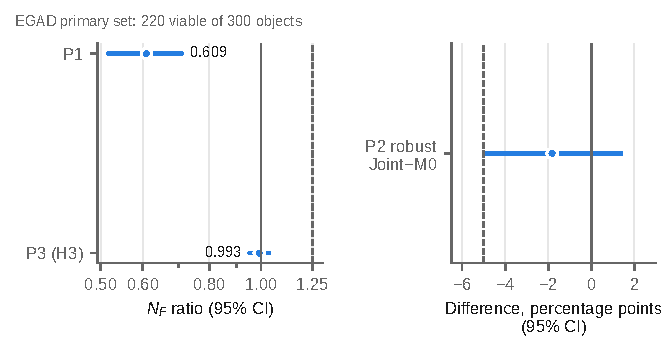
\includegraphics[width=\textwidth]{figures/fig_conf_primary.pdf}
\caption{Primary confirmatory contrasts on EGAD. Left: $N_F$ ratios (P1: Joint vs original planner; P3: Joint vs M1, dashed line = non-inferiority margin 1.25). Right: robustness difference Joint$-$M0 (dashed line = margin $-5$ percentage points).}\label{fig:conf}
\end{figure}

\paragraph{Secondary results.} None of the seven secondary hypotheses was supported (Supplementary Table~S2). The historical hypotheses did not replicate: M4 and M1 had the same load tolerance (\confSSoneEff), and M9 was not more robust than M1 (\confSStwoEff). Joint and M1 had the same load tolerance and robustness (\confSSthreeEff{} and \confSSfourEff). Joint was \emph{less} load tolerant than the original planner (\confSSfiveEff, failing the 10-point non-inferiority margin), the direction the articulated development pilot had suggested. The full online cost of Joint was \confSSsixEff{} times the original planner's (H4, Sect.~\ref{sec:cost}). The DINOv3 linear-branch MLP did not examine fewer candidates than the geometry MLP (\confSSsevenEff) nor than its permuted control (\confHfivePerm{} \confHfivePermCI); H5 was \confHfiveSupported.

\paragraph{Sensitivity.} The robustness non-inferiority holds only at the pre-registered torsional friction: the Joint$-$M0 robustness difference was \confTorLowPtwo{} \confTorLowPtwoCI{} at 0.001~m and \confTorHighPtwo{} \confTorHighPtwoCI{} at 0.02~m, both below zero. Across rotation thresholds it was \confRotFivePtwo{} (5$^\circ$), \confRotTenPtwo{} (10$^\circ$) and \confRotTwentyPtwo{} (20$^\circ$). With the articulated arm (\confArtObjects{} objects), Joint$-$M0 was \confArtJointMzeroRobust{} \confArtJointMzeroRobustCI{} in robustness (four standard conditions) and \confArtJointMzeroLoad{} \confArtJointMzeroLoadCI{} in load tolerance.

\paragraph{Fallback and negative transfer.} Joint examined more candidates than the original planner on \confNegJoint{} viable objects; the round-robin hybrid never exceeded twice the original planner's cost (\confHybridViol{} violations of the bound) and had geometric-mean $N_F$ \confHybridNF.

\paragraph{Evaluation set.} On the \evalViable{} viable of the \evalObjects{} EGAD evaluation-set objects (reported separately, not part of either family), Joint needed \evalNFJoint{} candidates against \evalNFMzero{} for the original planner, with equal robustness (\evalRobustJoint\% and \evalRobustMzero\%).

\begin{figure}[t]
\centering
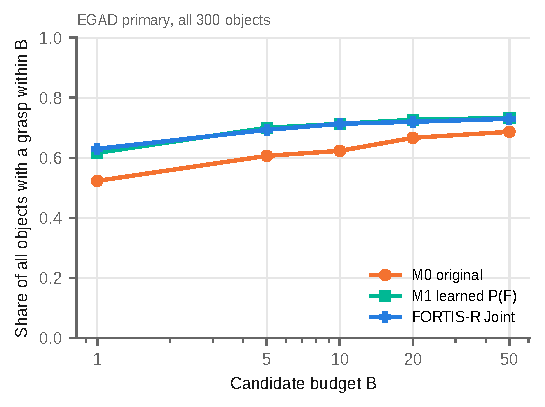
\includegraphics[width=0.55\textwidth]{figures/fig_conf_success_at_budget.pdf}
\caption{EGAD primary set, all \confObjects{} objects: share of objects for which a viable grasp is found within a budget of $B$ examined candidates. Objects without any viable candidate count as failures for every method.}\label{fig:success}
\end{figure}

\begin{table}[t]
\caption{EGAD primary set: all methods. $N_F$ on viable objects; S@1 and S@10 over all objects; v3 rates on viable objects with dynamics.}\label{tab:confmethods}
\centering\small
% Generated by make_tables.py
\begin{tabular}{lrrrrr}
\toprule
Method & $N_F$ & S@1 (\%) & S@10 (\%) & Robust v3 (\%) & Load v3 (\%) \\
\midrule
M0 & 2.09 & 52.3 & 62.3 & 92.7 & 85.0 \\
M1 & 1.28 & 61.7 & 71.3 & 91.8 & 77.7 \\
M4 & 1.29 & 62.7 & 71.0 & 90.0 & 77.7 \\
M9 & 1.26 & 62.3 & 72.0 & 90.9 & 75.4 \\
Joint & 1.27 & 63.0 & 71.3 & 90.9 & 78.6 \\
\bottomrule
\end{tabular}

\end{table}

\section{Online cost}\label{sec:cost}

The planner reports its own stage timings, and the full pipeline was timed from receiving an object to the planner's answer, with one thread and nothing else running. In the current implementation the learned orders need the candidates before planning, so candidate generation runs twice: once in a separate export process and once inside the planner. On \timeObjects{} confirmatory objects the median full cost was \timeMzero~s for the original planner and \timeJoint~s for Joint. Generation alone took \timeGen~s, whereas the search stage that the order accelerates took \timeSearchMzero~ms (original) and \timeSearchJoint~ms (Joint); every first grasp of the timed runs matched the order replay (\timeMismatch{} mismatches). On \costParts{} development parts the full-cost ratio was \costJointTotal{} \costJointTotalCI; subtracting the duplicated generation---an engineering estimate of a single-process implementation, not a measurement---gives \costJointIntegrated{} \costJointIntegratedCI. A visual prior would add rendering (\costDinoRender~s median for 16 views on CPU) and encoding (\costDinoEncode~s). The classical analytic order (force closure, then wrench-space quality \cite{ferrari1992planning}), evaluated on \epsParts{} development parts, needed \epsNF{} candidates against \epsNFMzero{} for the original planner and \epsNFJoint{} for Joint, and its quality export took \epsSeconds~s per part.
